\chapter{Experimenty}

V predchádzajúcej kapitole sme uviedli množstvo parametrov, ktoré ovplyvňujú rôzne časti nášho algoritmu. Ich hodnoty sa nedajú nijako vypočítať, ale vieme im určiť rozumné hranice a následne experimentálne vybrať tú najlepšiu možnosť. Získané hodnoty parametrov potom použijeme na porovnanie nášho algoritmu s nástrojom LoRMA.

\section{Jadrá korekcie}

V tejto časti uvedieme výsledky, ako vplývajú parametre hľadania jadier zarovnania na ich kvalitu a na pokrytie čítania jadrami. Kedže upravené čítania sú reťazce pospájaných jadier korekcie, pokrytie čítania jadrami je nutná podmienka pre fungovanie korekcie. Na druhej strane príliš voľné podmienky spôsobia, že vysoký počet falošných jadier zarovnania bude výrazne predlžovať výpočet.

Detekciu jadier korekcie ovplyvňujú tieto parametre:

\begin{enumerate}[label={P.\arabic*}]
\item \label{dlzka_kmerov} Minimálna dĺžka zhody medzi čítaniami
\item \label{absolutny_clen} Minimálny súčet dĺžok zhôd medzi prekrývajúcimi sa čítaniami (absolútny člen funkcie)
\item \label{linearny_clen} Podiel dĺžky prekrytia, ktorý pripočítavame k minimálnemu súčtu dĺzok (lineárny člen funkcie)
\end{enumerate}

Pri rôznych kombináciách týchto parametrov pozorujeme, ako sa mení čas výpočtu a kvalita výslednej sekvencie. Kvalitu posudzujeme zarovnávaním sekvencií na genóm pomocou nástroja BLASR. 

\begin{table}
    \fontsize{11}{13}\selectfont
    \centering
    \begin{tabular}{ | l || c | c | c | }
    \hline 
& 0.001& 0.005& 0.01 \\ \hline \hline
30 & 92.69\%; 4.59 s; 82.81\% & 92.65\%; 4.31 s; 82.88\% & 92.77\%; 4.34 s; 82.84\% \\ \hline
40 & 92.71\%; 4.69 s; 82.74\% & 92.76\%; 4.43 s; 82.80\% & 92.27\%; 4.28 s; 82.92\% \\ \hline
50 & 92.39\%; 4.41 s; 82.81\% & 92.34\%; 4.43 s; 82.82\% & 92.15\%; 4.63 s; 82.86\% \\ \hline
60 & 92.35\%; 4.35 s; 82.83\% & 93.03\%; 4.24 s; 80.88\% & 92.87\%; 4.10 s; 80.29\% \\ \hline
80 & 93.05\%; 4.26 s; 80.24\% & 92.80\%; 4.21 s; 80.23\% & 92.96\%; 3.88 s; 80.16\% \\ \hline
    \end{tabular}
    \caption{Zhoda s genómom, čas opravy jedného čítania a podiel dĺžky výstupu/vstupu pre dĺžku jadier korekcie \ref{dlzka_kmerov}$ = 13$ a rôzne hodnoty parametrov \ref{absolutny_clen} (riadky) a \ref{linearny_clen} (stĺpce)}
    \label{exp_jadra_k13}
\end{table}

\begin{table}
    \fontsize{11}{13}\selectfont
    \centering
    \begin{tabular}{ | l || c | c | c | }
    \hline 
& 0.001& 0.005& 0.01 \\ \hline \hline
30 & 92.07\%; 4.70 s; 81.04\% & 92.68\%; 4.21 s; 79.82\% & 92.81\%; 4.03 s; 78.94\% \\ \hline
40 & 92.43\%; 4.35 s; 80.26\% & 92.79\%; 3.99 s; 78.90\% & 92.98\%; 3.77 s; 78.37\% \\ \hline
50 & 92.85\%; 3.97 s; 78.85\% & 92.88\%; 3.85 s; 78.56\% & 92.88\%; 3.67 s; 78.17\% \\ \hline
60 & 92.89\%; 3.89 s; 78.58\% & 92.85\%; 3.84 s; 78.61\% & 92.97\%; 3.77 s; 77.45\% \\ \hline
80 & 92.94\%; 3.81 s; 77.88\% & 92.66\%; 4.11 s; 77.40\% & 92.54\%; 3.78 s; 77.35\% \\ \hline
    \end{tabular}
    \caption{Zhoda s genómom, čas opravy jedného čítania a podiel dĺžky výstupu/vstupu pre dĺžku jadier korekcie \ref{dlzka_kmerov}$ = 14$ a rôzne hodnoty parametrov \ref{absolutny_clen} (riadky) a \ref{linearny_clen} (stĺpce)}
    \label{exp_jadra_k14}
\end{table}

\begin{table}
    \fontsize{11}{13}\selectfont
    \centering
    \begin{tabular}{ | l || c | c | c | }
    \hline 
& 0.001& 0.005& 0.01 \\ \hline \hline
30 & 90.91\%; 3.94 s; 78.72\% & 91.74\%; 3.78 s; 76.21\% & 91.56\%; 3.54 s; 76.52\% \\ \hline
40 & 91.17\%; 3.82 s; 77.43\% & 91.56\%; 3.57 s; 76.46\% & 91.68\%; 3.53 s; 75.74\% \\ \hline
50 & 91.39\%; 3.60 s; 76.40\% & 91.68\%; 3.43 s; 75.73\% & 91.71\%; 3.46 s; 75.68\% \\ \hline
60 & 91.54\%; 3.48 s; 75.72\% & 91.68\%; 3.35 s; 75.73\% & 91.68\%; 3.35 s; 75.66\% \\ \hline
80 & 91.35\%; 3.46 s; 75.65\% & 90.80\%; 3.19 s; 75.63\% & 91.56\%; 3.00 s; 72.83\% \\ \hline
    \end{tabular}
    \caption{Zhoda s genómom, čas opravy jedného čítania a podiel dĺžky výstupu/vstupu pre dĺžku jadier korekcie \ref{dlzka_kmerov}$ = 15$ a rozne hodnoty parametrov \ref{absolutny_clen} (riadky) a \ref{linearny_clen} (stĺpce)}
    \label{exp_jadra_k15}
\end{table}

V tabuľkách \ref{exp_jadra_k13}, \ref{exp_jadra_k14} a \ref{exp_jadra_k15} sú uvedené výsledky experimentov s parametrami hľadania jadier korekcie. Na zvislej osi sú hodnoty parametra \ref{absolutny_clen} a na vodorovnej hodnoty parametra \ref{linearny_clen}. Rozdiely sú síce prekvapivo malé, ale zistili sme, že na dosiahnutie najvyššej kvality korekcie je vhodné nastaviť \ref{absolutny_clen} na 60 a \ref{linearny_clen} na 0,005. Zvyšovanie týchto parametrov vedie ku skráteniu času korekcie, avšak poklesu dĺžky výstupu.


\section{Graf jadier}

V súvislosti s vytváraním grafu jadier korekcie sme v predchádzajúcej kapitole uviedli tri heuristické metódy na zníženie počtu hrán. Najprv otestujeme metódu obmedzenia očakávanej vzdialenosti medzi jadrami korekcie. Za predpokladu, že očakávaná pozícia sa veľmi nelíši od skutočnej pozície na čítaní, by sa mala dať nájsť hranica, ktorá urýchli výpočet ale na kvalite zarovnania sa neprejaví.

\begin{figure}
    \centering
    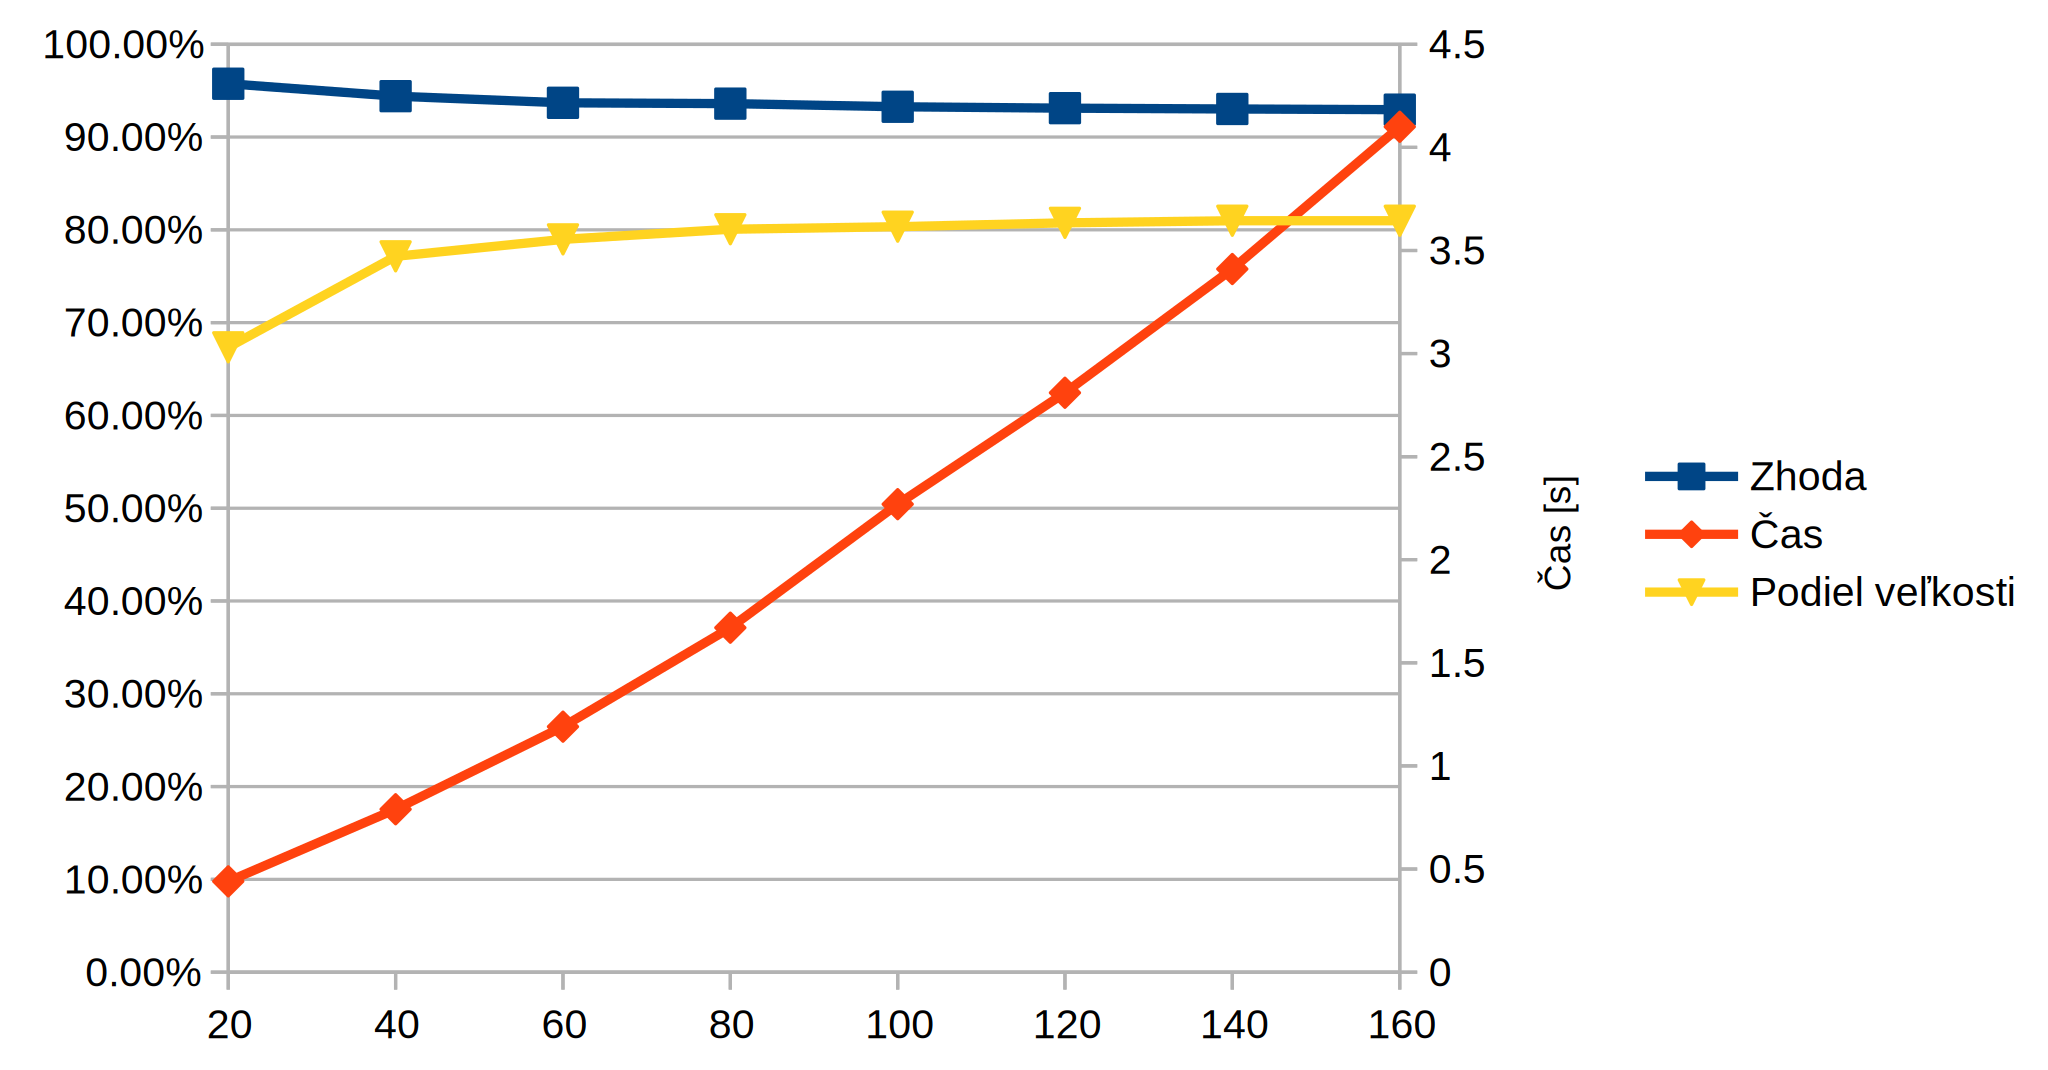
\includegraphics[width=0.8\textwidth]{images/max_node_distance.png}
    \caption{Vplyv maximálnej očakávanej vzdialenosti susedných jadier v grafe na kvalitu korekcie}
    \label{fig:max_node_distance}
\end{figure} 

Graf \ref{fig:max_node_distance} ukazuje ako sa vlastnosti opravených čítaní menia, ked meníme maximálnu očakávanú vzdialenosť medzi jadrami korekcie na vytvorenie hrany. Zistili sme, že hodnota 80 nezhorší veľkosť výstupu ani zhodu opravených sekvencií s genómom. Priemerný čas opravy jedného čítania sa ale zníži na menej ako polovicu oproti hranici 160. Pri testovaní zvyšných metód použijeme bezpečnú hranicu 100.


\begin{figure}
    \centering
    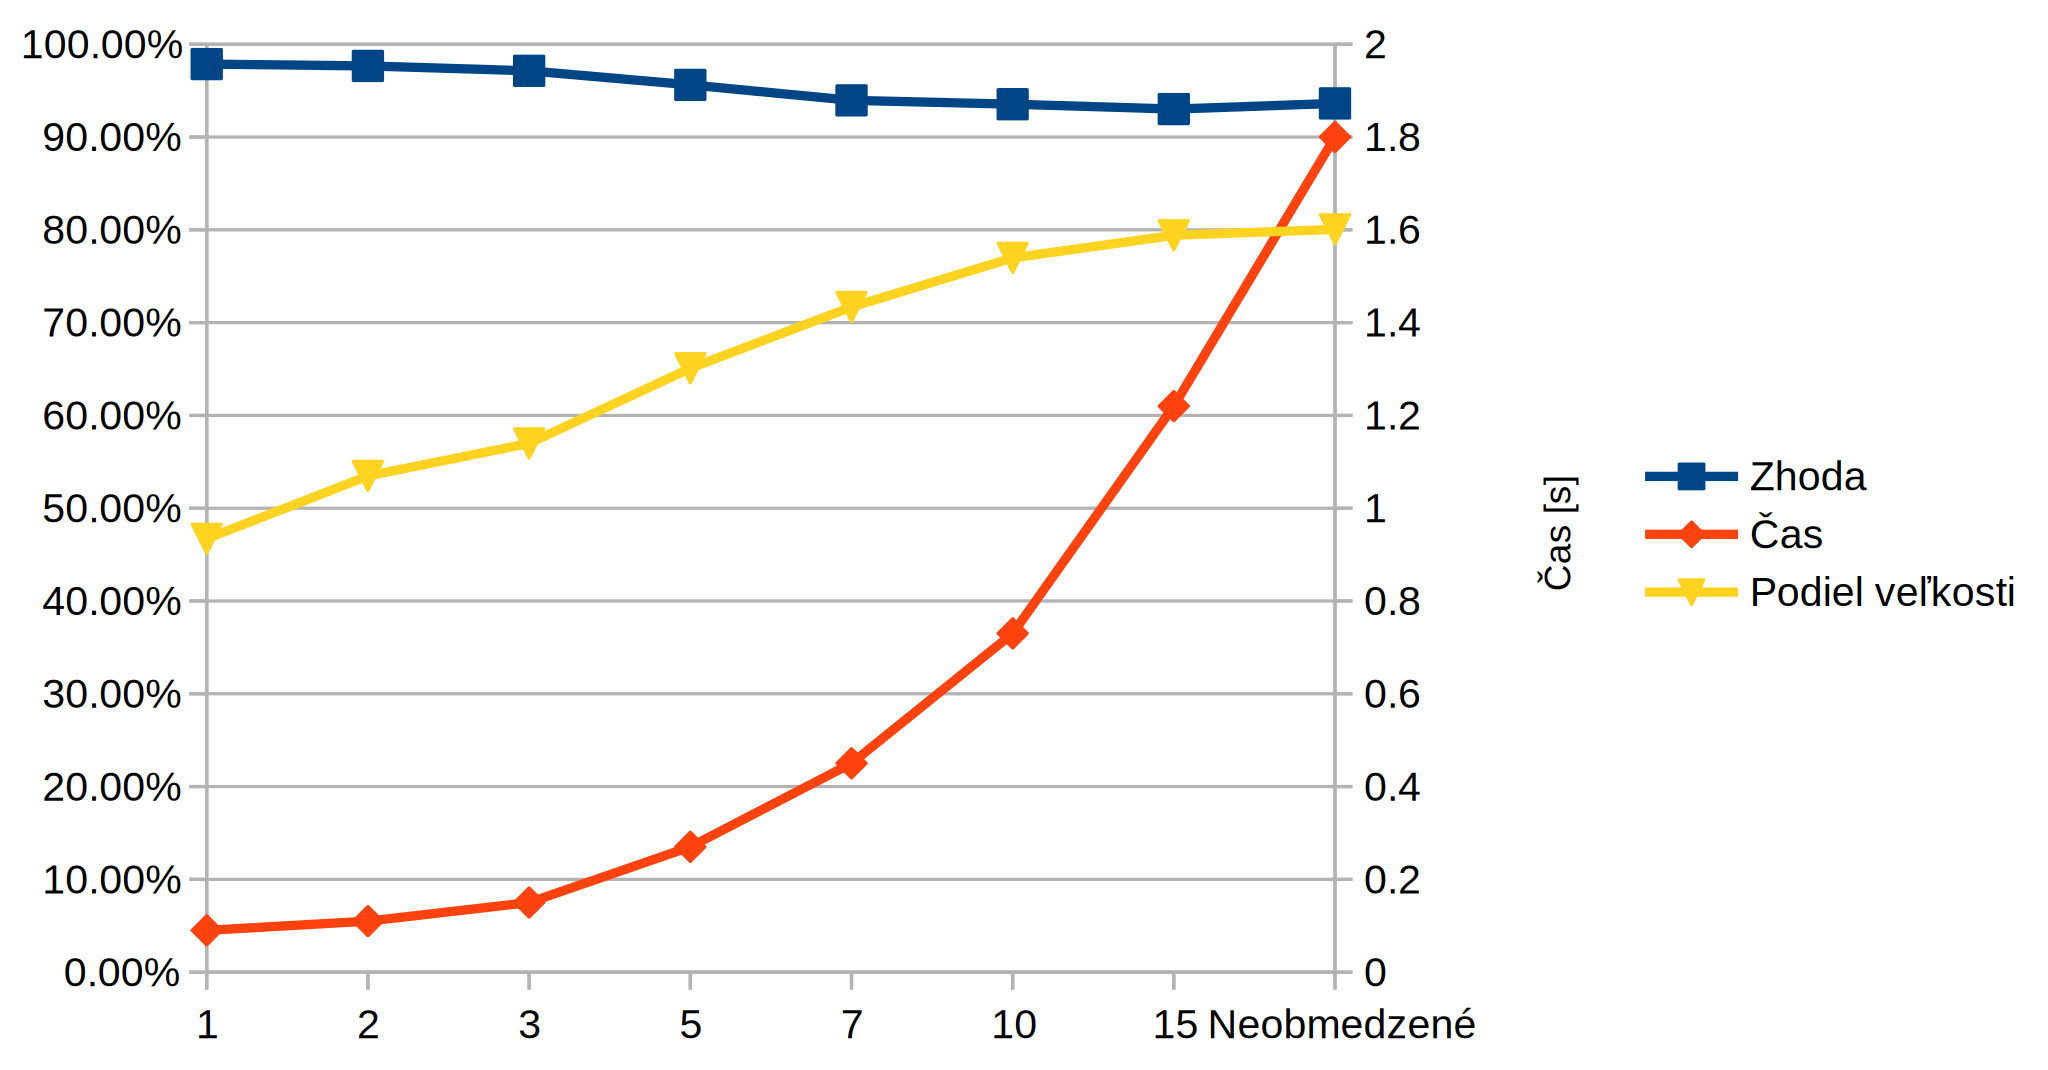
\includegraphics[width=0.8\textwidth]{images/max_edges_from_node.png}
    \caption{Vplyv maximálneho počtu hrán z jadra korekcie v grafe jadier na kvalitu korekcie}
    \label{fig:max_edges_from_node}
\end{figure} 

\begin{figure}
    \centering
    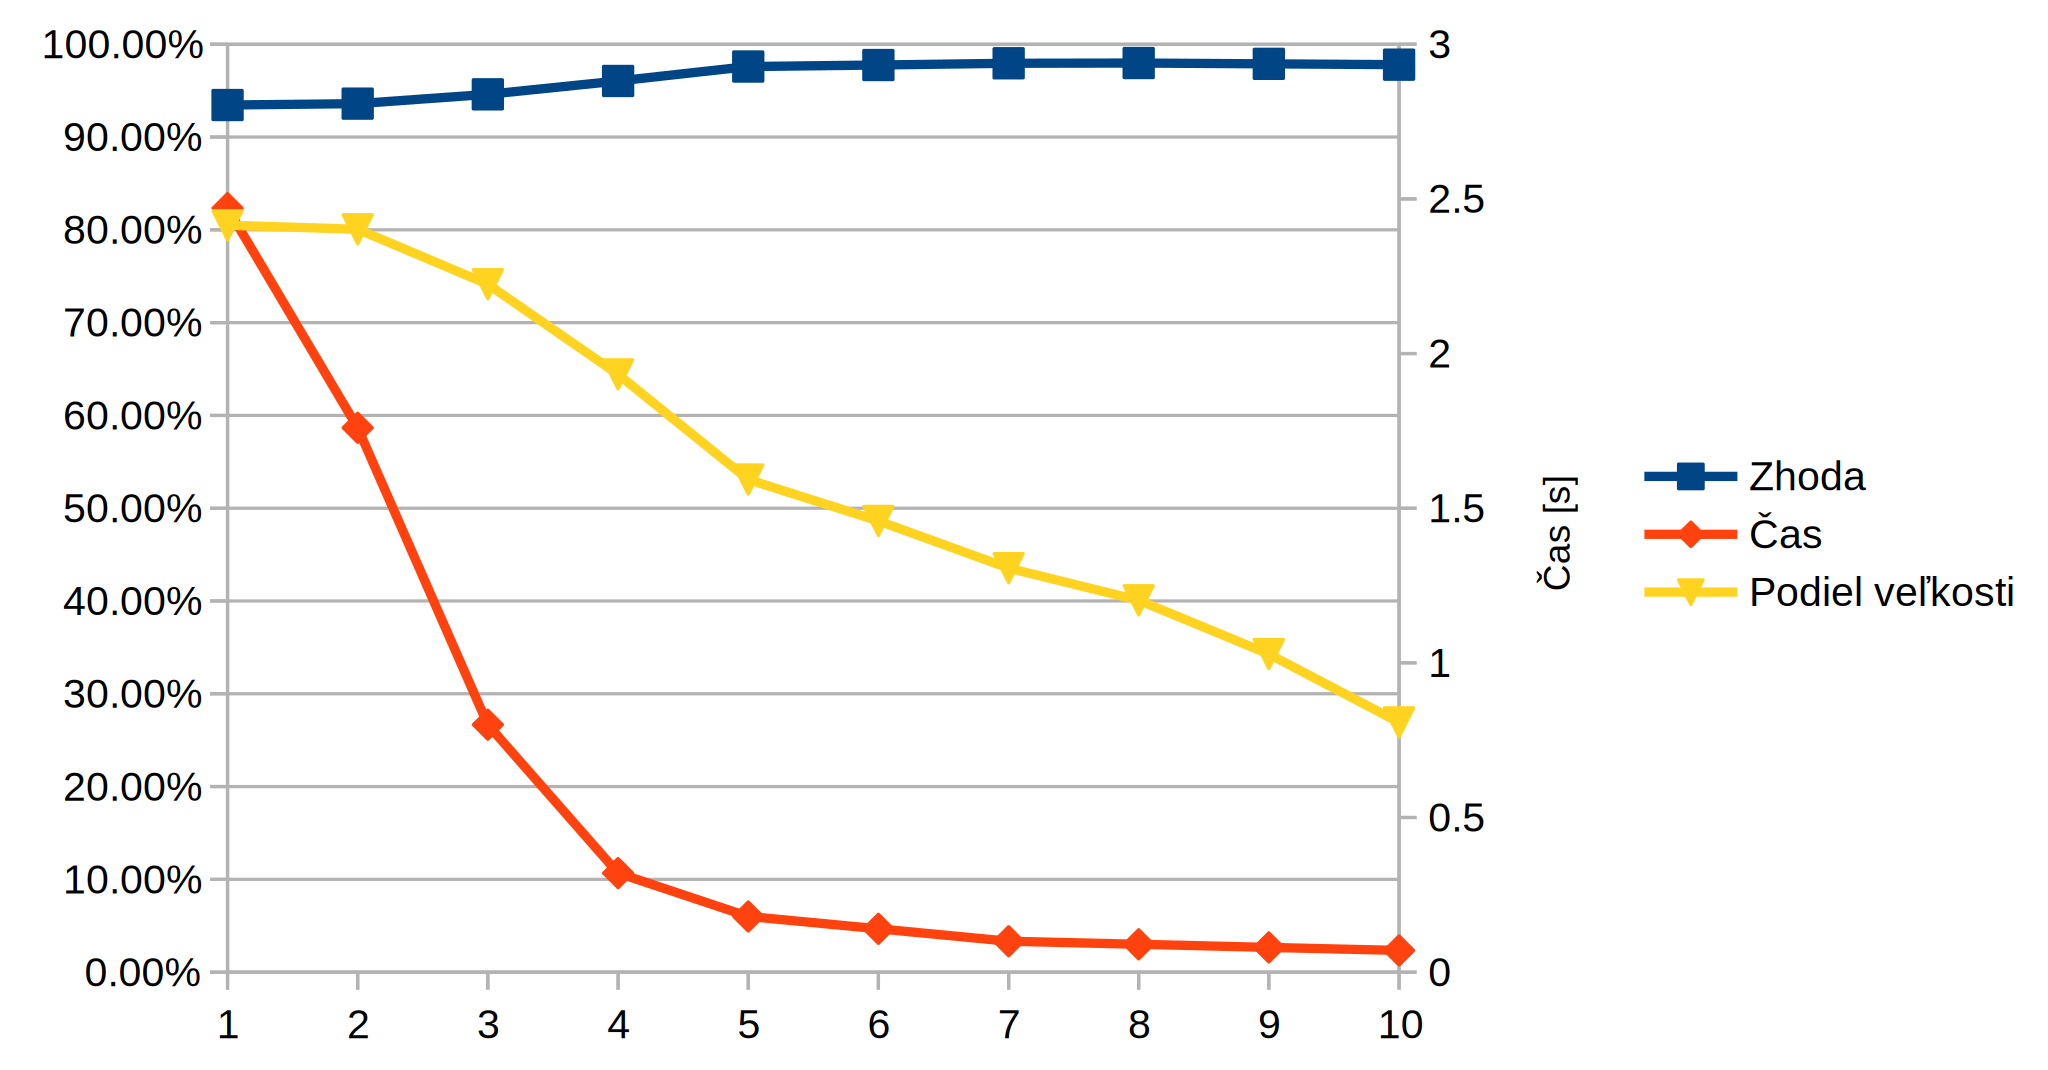
\includegraphics[width=0.8\textwidth]{images/min_node_overlap.png}
    \caption{Vplyv minimálneho prekrytia susedných jadier korekcie v grafe jadier na kvalitu korekcie}
    \label{fig:min_node_overlap}
\end{figure} 

Teraz sa pozrieme na vplyv zvyšných dvoch metód. Výsledky sú zhrnuté v grafoch \ref{fig:max_edges_from_node} a \ref{fig:min_node_overlap}. Ukazuje sa, že obe metódy už pri miernych nastaveniach znižujú podiel výstupných dát. Závisí však, čo od nástroja očakávame. Sprísnením týchto parametrov sa okrem skrátenia času zlepší aj zhoda výslednej sekvencie s genómom a to môže byť niekedy prioritnejšie.


\section{Penalizácia}

Ako sme uviedli v predchádzajúcej kapitole, penalizáciu vieme použiť na zvýšenie priemerného prekrytia po sebe idúcich jadier korekcie. Vyskúšali sme niekoľko jednoduchých funkcií na výpočet penalizácie z dĺžky prekrytia. Výsledky sme uviedli v tabuľke \ref{penalizacia_za_prekrytie}. Ukázalo sa, že najlepšie výsledky dosahujeme pri použití funkcie $x^2/5$.

\begin{table}[H]
    \fontsize{11}{13}\selectfont
    \centering
    \begin{tabular}{ | l || c | c | c | }
    \hline 
Funkcia& Zhoda s genómom & Čas [s] & Podiel veľkosti \\ \hline \hline
$0$ & 92.70\% & 2.25 & 79.98\% \\ \hline
$x/8$ & 92.76\% & 2.47 & 80.04\% \\ \hline
$x/5$ & 92.99\% & 2.43 & 80.08\% \\ \hline
$x/3$ & 93.15\% & 2.54 & 79.95\% \\ \hline
$x$ & 93.88\% & 2.48 & 79.83\% \\ \hline
$x^2/10$ & 93.96\% & 2.13 & 79.92\% \\ \hline
$x^2/8$ & 94.07\% & 2.20 & 79.99\% \\ \hline
$x^2/5$ & 94.07\% & 1.92 & 79.99\% \\ \hline
$x^2/3$ & 93.96\% & 1.68 & 80.24\% \\ \hline
    \end{tabular}
    \caption{Vplyv penalizácie za veľkosť prekrytia na kvalitu korekcie. Premenná $x$ je posunutie cieľového jadra korekcie oproti východziemu v ich prekrytí}
    \label{penalizacia_za_prekrytie}
\end{table}

Ďalšia možnosť využitia penalizácie je pomocou nej udžiavať jadrá korekcie blízko svojej očakávanej pozície. Na grafe \ref{fig:max_node_misplacement} je zobrazené, ako sa menia vlastnosti korekcie, keď meníme veľkosti intervalov, v ktorých sa jadrá korekcie môžu nachádzať. Z výsledkov vyplýva, že zhoda s genómom a podiel veľkosti výstupu sa mení minimálne. Nastavením maximálnej vzdialenosti na hodnotu 40 vieme znížiť čas výpočtu o 25\%.

\begin{figure}
    \centering
    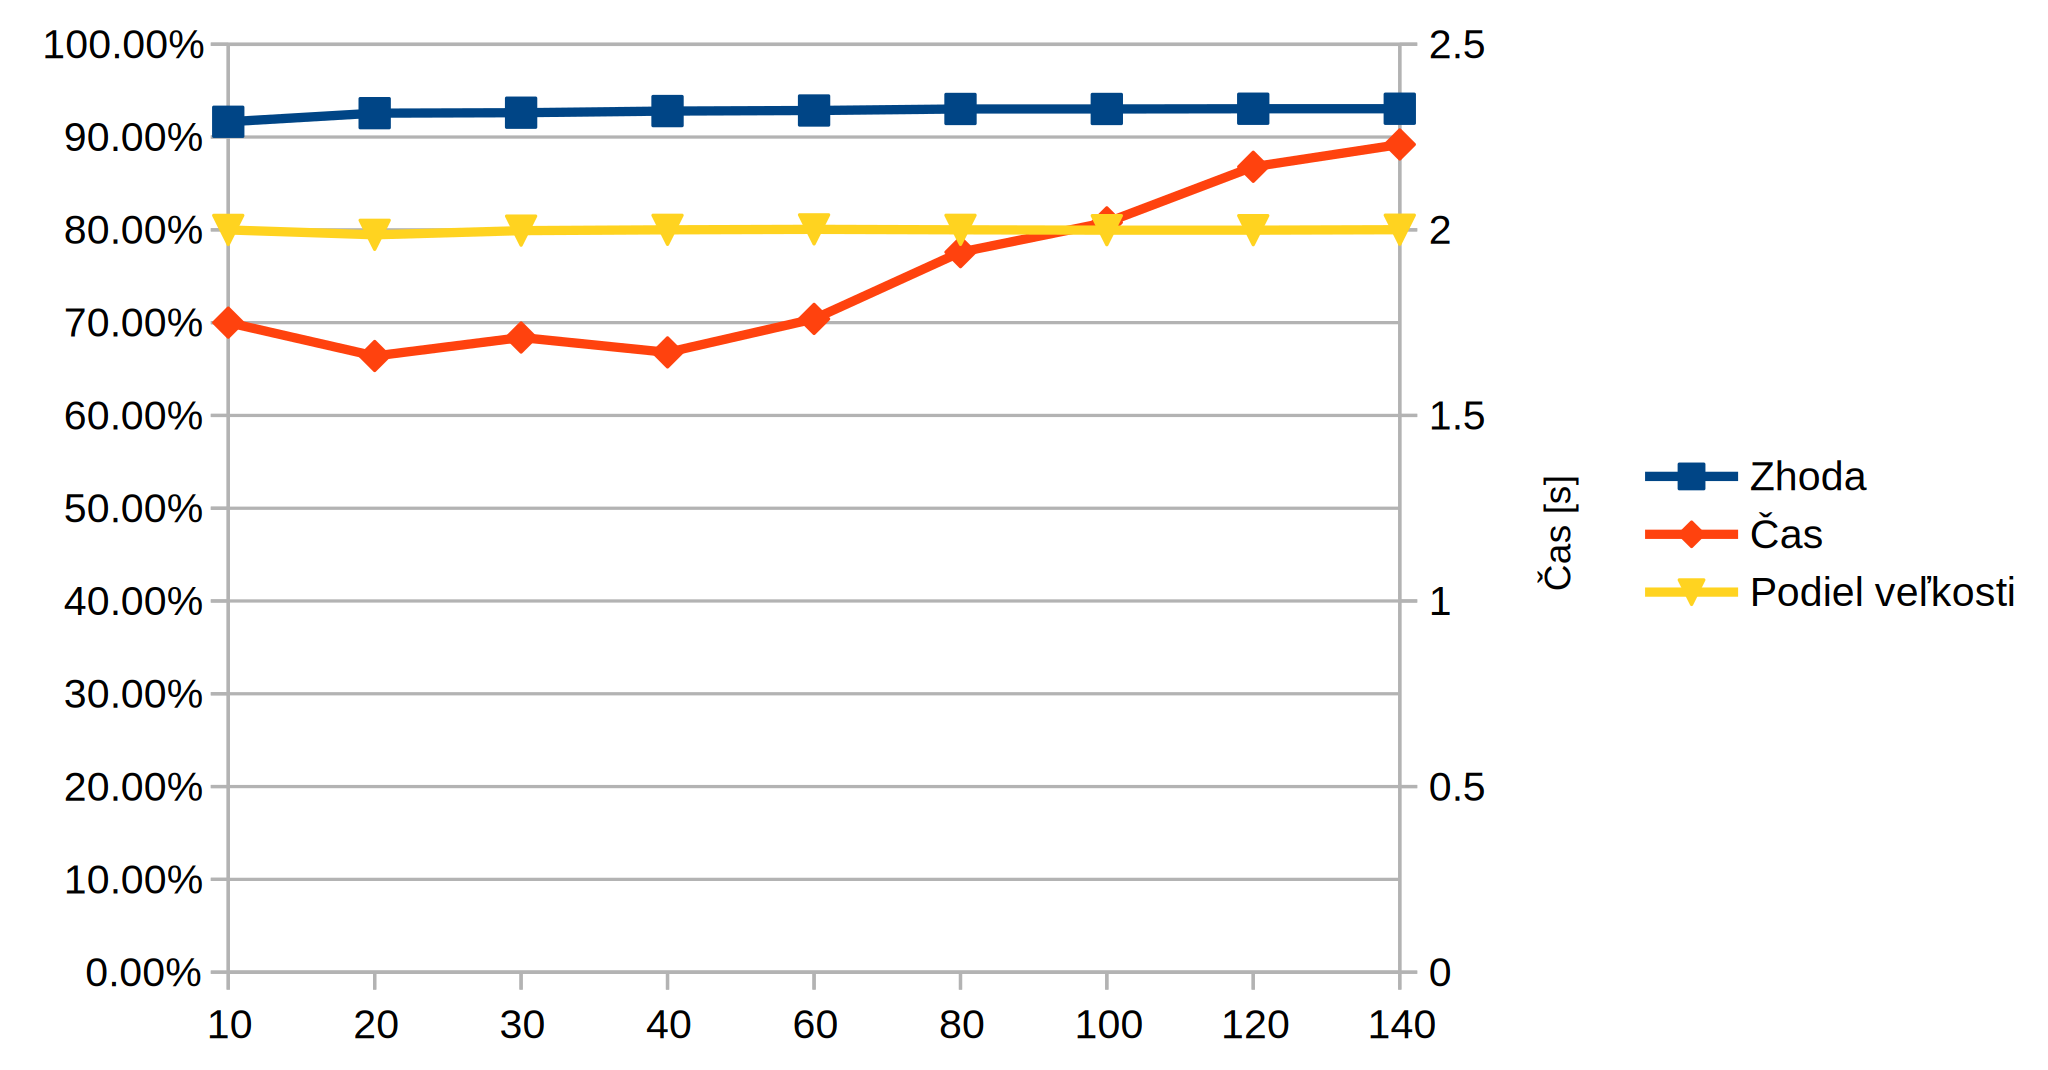
\includegraphics[width=0.8\textwidth]{images/max_node_misplacement.png}
    \caption{Vplyv maximálnej vzdialenosti umiestnenia jadra korekcie od očakávanej pozície na kvalitu korekcie}
    \label{fig:max_node_misplacement}
\end{figure} 

\section{Heuristiky rekonštrukcie}

Prvou uvedenou heuristikou pri rekonštrukcii bolo zahadzovanie vetiev výpočtu, ktoré v rámci čítania zaostávajú za doteraz najďalej siahajúcou vetvou o viac ako $d$ báz. Jej vplyv je zobrazený na grafe \ref{fig:max_distance_from_furthest_reaching}. Ukazuje sa, že parameter $d$ môžeme znížiť až na hodnotu 15 a kvalita korekcie sa tým vôbec nezhorší. Priemerný čas korekcie pri tom klesne až o 70\%.

\begin{figure}
    \centering
    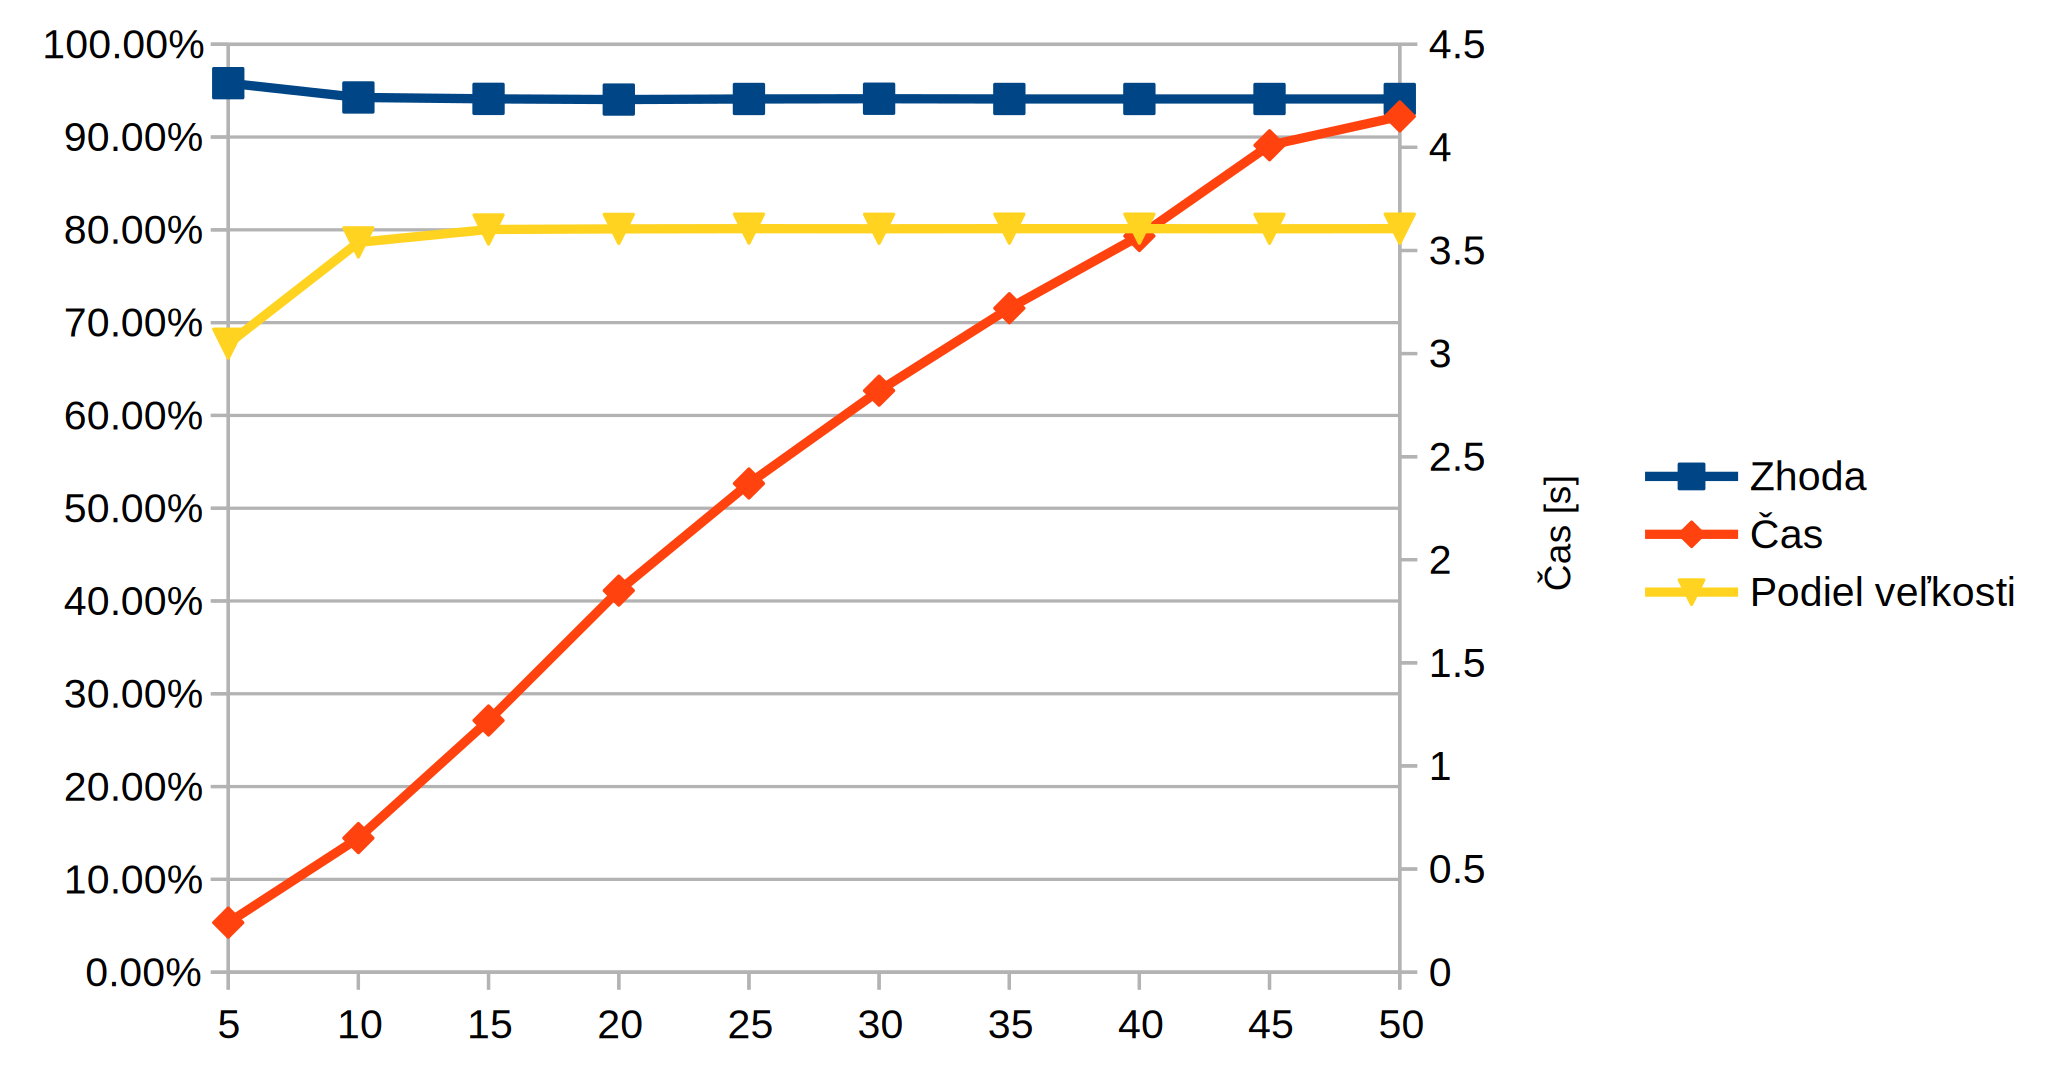
\includegraphics[width=0.8\textwidth]{images/max_distance_from_furthest_reaching.png}
    \caption{Vplyv heuristickej metódy, ktorá zahadzuje vetvy príliš zaostávajúce za najdalej siahajúcou vetvou. Na vodorovnej osi je parameter $d$}
    \label{fig:max_distance_from_furthest_reaching}
\end{figure} 

Ďalšou uvedenou heuristickou metódou bolo udržiavanie lokálnej zhody generovanej sekvencie so zodpovedajúcim úsekom čítania. V tejto metóde vystupujú dva parametre: veľkosť okna, ktorom zhody počítame, $d$ a minimálny počet zhod $m$ za posledných $d$ báz. Podľa výsledkov v tabuľke \ref{local_match_rate} môžeme usúdiť, že menšie veľkosti okna poozitívne vplývajú na čas výpočtu. Parameter $m$ nastavíme podľa toho, či uprednostňujeme vyššiu zhodu s genómom, alebo vyšší podiel výstupných dát.

\begin{table}
    \fontsize{11}{13}\selectfont
    \centering
    \begin{tabular}{ | l | l || c | c | c | }
    \hline 
$d$ & $m$ & Zhoda s genómom & Čas [s] & Podiel veľkosti \\ \hline \hline
15 & 8 & 93.46\% & 1.72 & 79.79\% \\ \hline
15 & 9 & 94.89\% & 0.75 & 74.50\% \\ \hline
15 & 10 & 96.34\% & 0.41 & 66.65\% \\ \hline
20 & 11 & 93.65\% & 1.94 & 79.96\% \\ \hline
20 & 12 & 94.24\% & 1.47 & 78.07\% \\ \hline
20 & 13 & 95.85\% & 0.78 & 72.63\% \\ \hline
20 & 14 & 96.68\% & 0.51 & 64.99\% \\ \hline
30 & 16 & 93.58\% & 2.87 & 79.12\% \\ \hline
30 & 17 & 93.88\% & 2.46 & 79.28\% \\ \hline
30 & 18 & 94.22\% & 2.17 & 78.66\% \\ \hline
    \end{tabular}
    \caption{Vplyv heuristickej metódy, ktorá od vetiev vyžaduje minimálne $m$ zhôd za posledných $d$ báz}
    \label{local_match_rate}
\end{table}

\section{Porovnanie s nástrojom LoRMA}

Aby sme mohli porovnať náš algoritmus s nástrojom LoRMA, vyrobili sme vstupné dáta s vyšším pokrytím. Zarovnali sme množinu čítaní DNA baktérie E. coli so stonásobným pokrytím na referenčný genóm. Zvolili sme si úsek genómu dlhý 100 000 báz a vybrali sme toľko čítaní prekrývajúcich sa s vybraným úsekom, aby bolo priemerné pokrytie 50.
Na týchto dátach sme spustili oba nástroje. Nástroj lorma bol spustený so prednastavenými parametrami na jednom vlákne. Parametre nášho nástroja sme nastavili v prostech rýchlosti výpočtu. Po dokončení prvého chodu sme náš nástroj spustili ešte raz na výstup z prvého chodu s vyšším parametrom dĺžky jadier (\ref{dlzka_kmerov}). Výsledky sú uvedene v tabuľke \ref{porovnanie_s_lormou}.

\begin{table}
    \centering
    \begin{tabular}{ | l || c | c | c | }
    \hline 
& LoRMA & Náš algoritmus & Druhá iterácia \\ \hline \hline
Čas & 23,078 s & 739,667 s & +287.851 s \\ \hline
Zhoda s genómom (\%) & 98,72 & 94,60 & 95,56 \\ \hline
Veľkosť výstupu (\%) & 5,22 & 50,13 & 41,96 \\ \hline
    \end{tabular}
    \caption{Porovnanie kvality a rýchlosti zarovnávania nášho algoritmu s nástrojom LoRMA}
    \label{porovnanie_s_lormou}
\end{table}

Ukázalo sa, že náš algoritmus je výrazne pomalší a výstupné sekvencie majú vyššiu mieru chýb. Na druhej strane veľkosť výstupu je pri danom pokrytí skoro 10 krát vyššia ako z nástroja LoRMA.